\section{Principle Component Analysis (PCA)}
There are many different approaches to identify music by extracting different audio features as
discussed in the Chapter \ref{chapter:lit_review}. Since there are very low number of researches
conducted on sinhala music identification, finding audio features which can differentiate two 
sinhala songs was required to continue the research. Hence \ac{pca} was conducted to find features
on a 5000 song dataset extracting 27 different audio features and results were collected for 
different normalization techniques. \ac{svd} is used to composite multi-dimension features.

\subsection{PCA with Raw Dataset}



\begin{figure}[H]
    \centering
    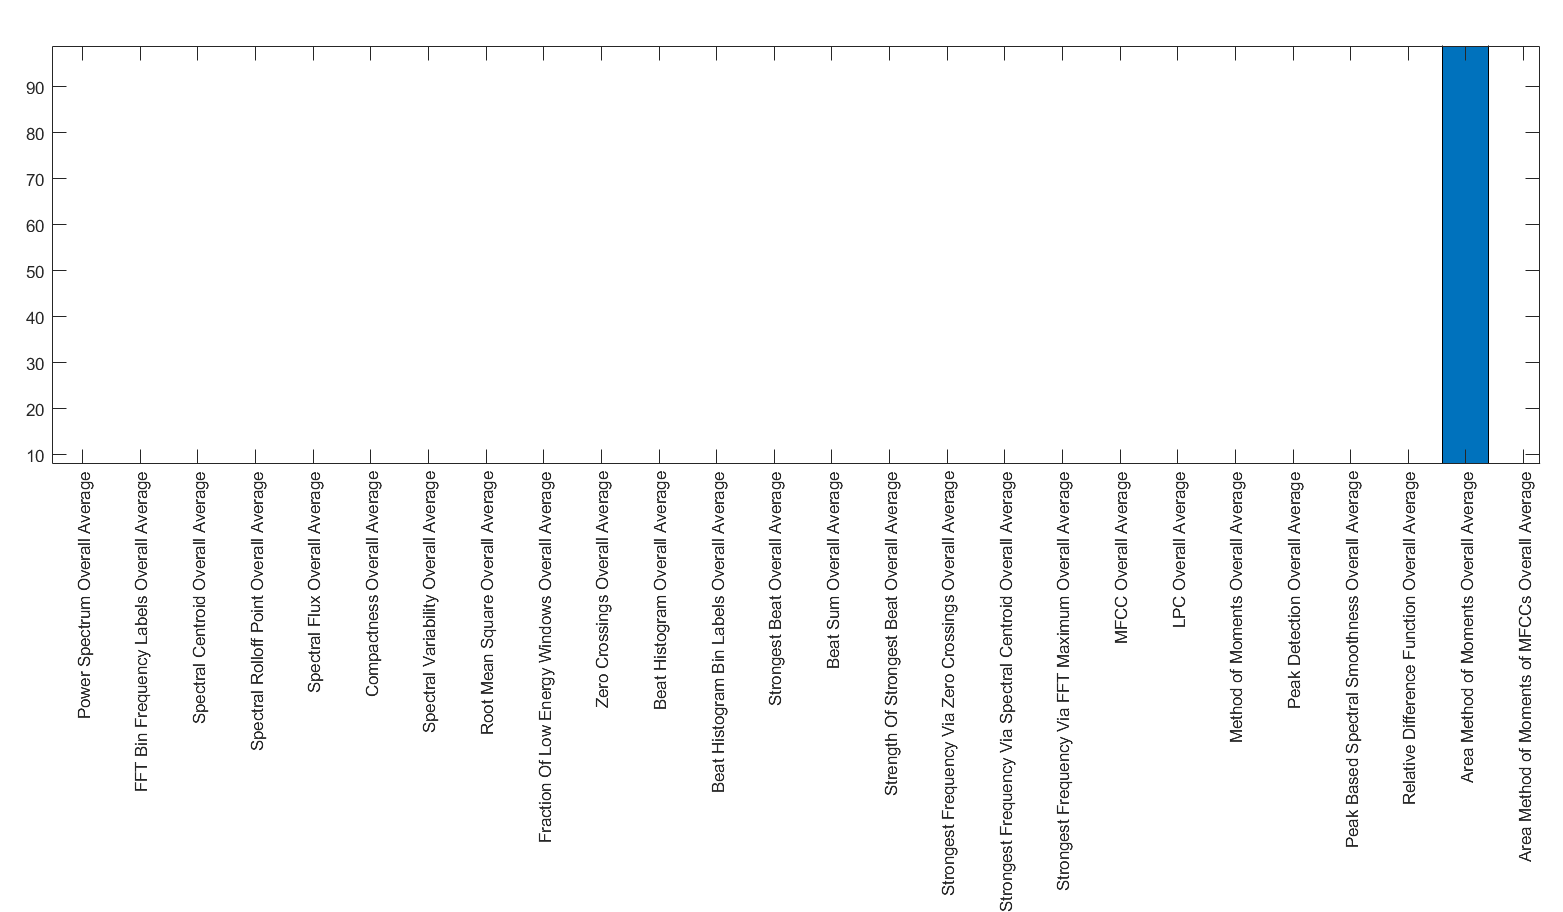
\includegraphics[scale=0.35]{pca_coeff.png}
    \caption{PCA coefficients weighted by eigen values}
    \label{fig:pca_coeff}
\end{figure}

\subsection{PCA with Dataset Normalized by Z-score}
\begin{figure}[H]
    \centering
    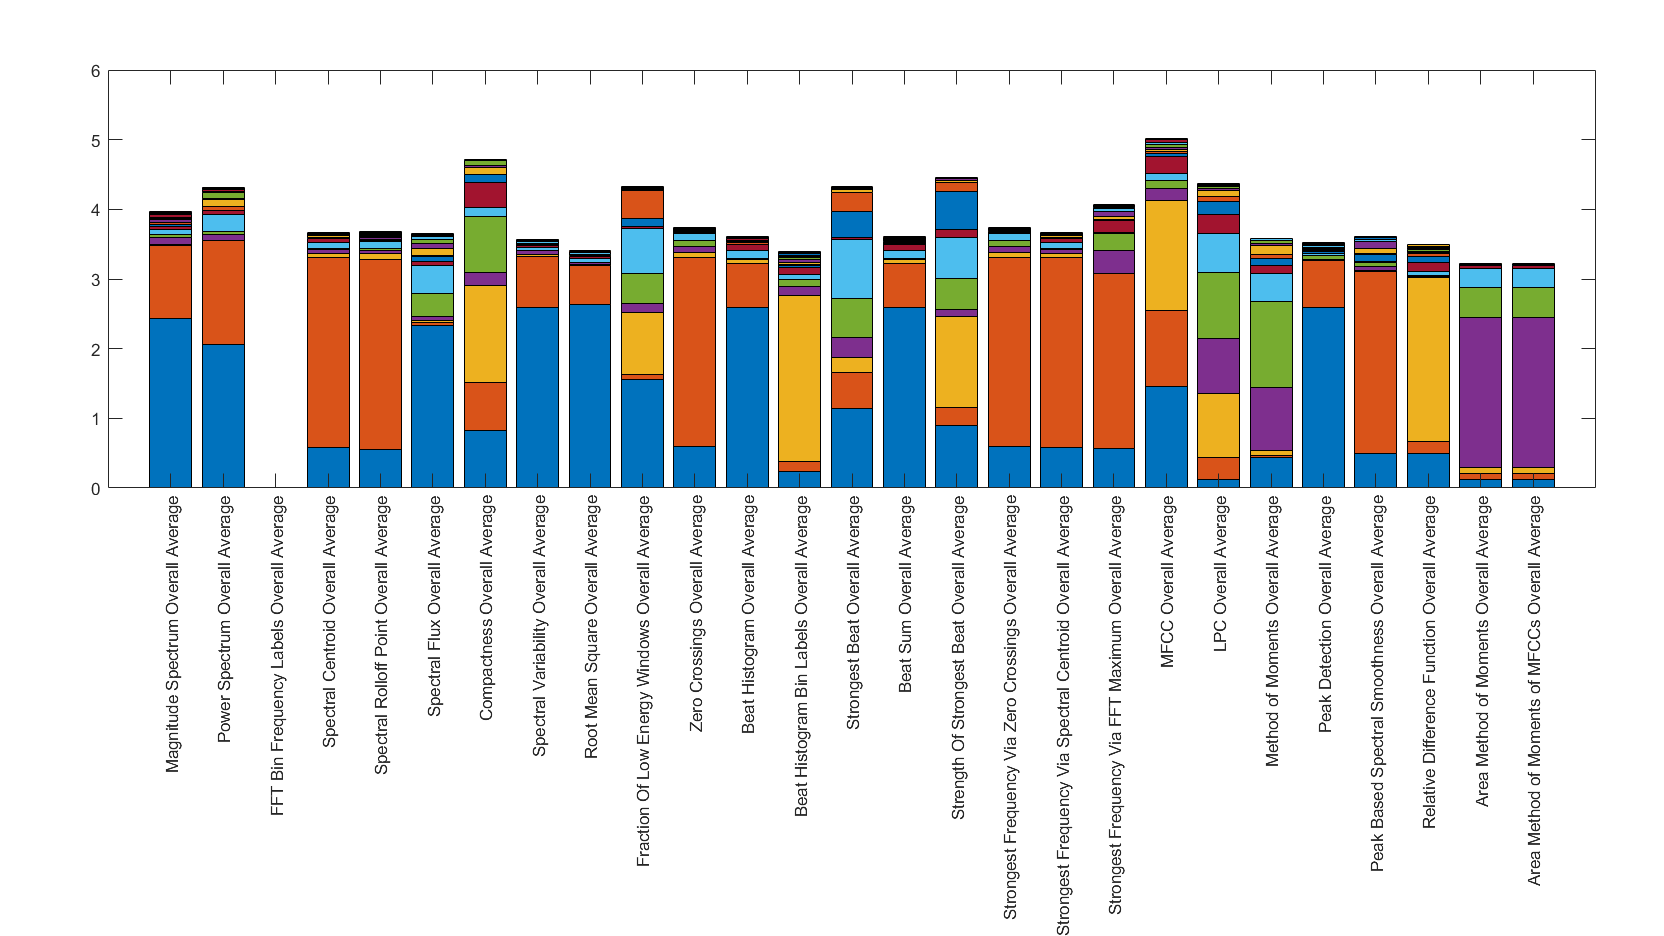
\includegraphics[scale=0.35]{pca_coeff_z.png}
    \caption{PCA coefficients weighted by eigen values (Normalized by Zscore)}
    \label{fig:pca_coeff_z}
\end{figure}

\subsection{PCA with Dataset Normalized by Rescaling}
\begin{figure}[H]
    \centering
    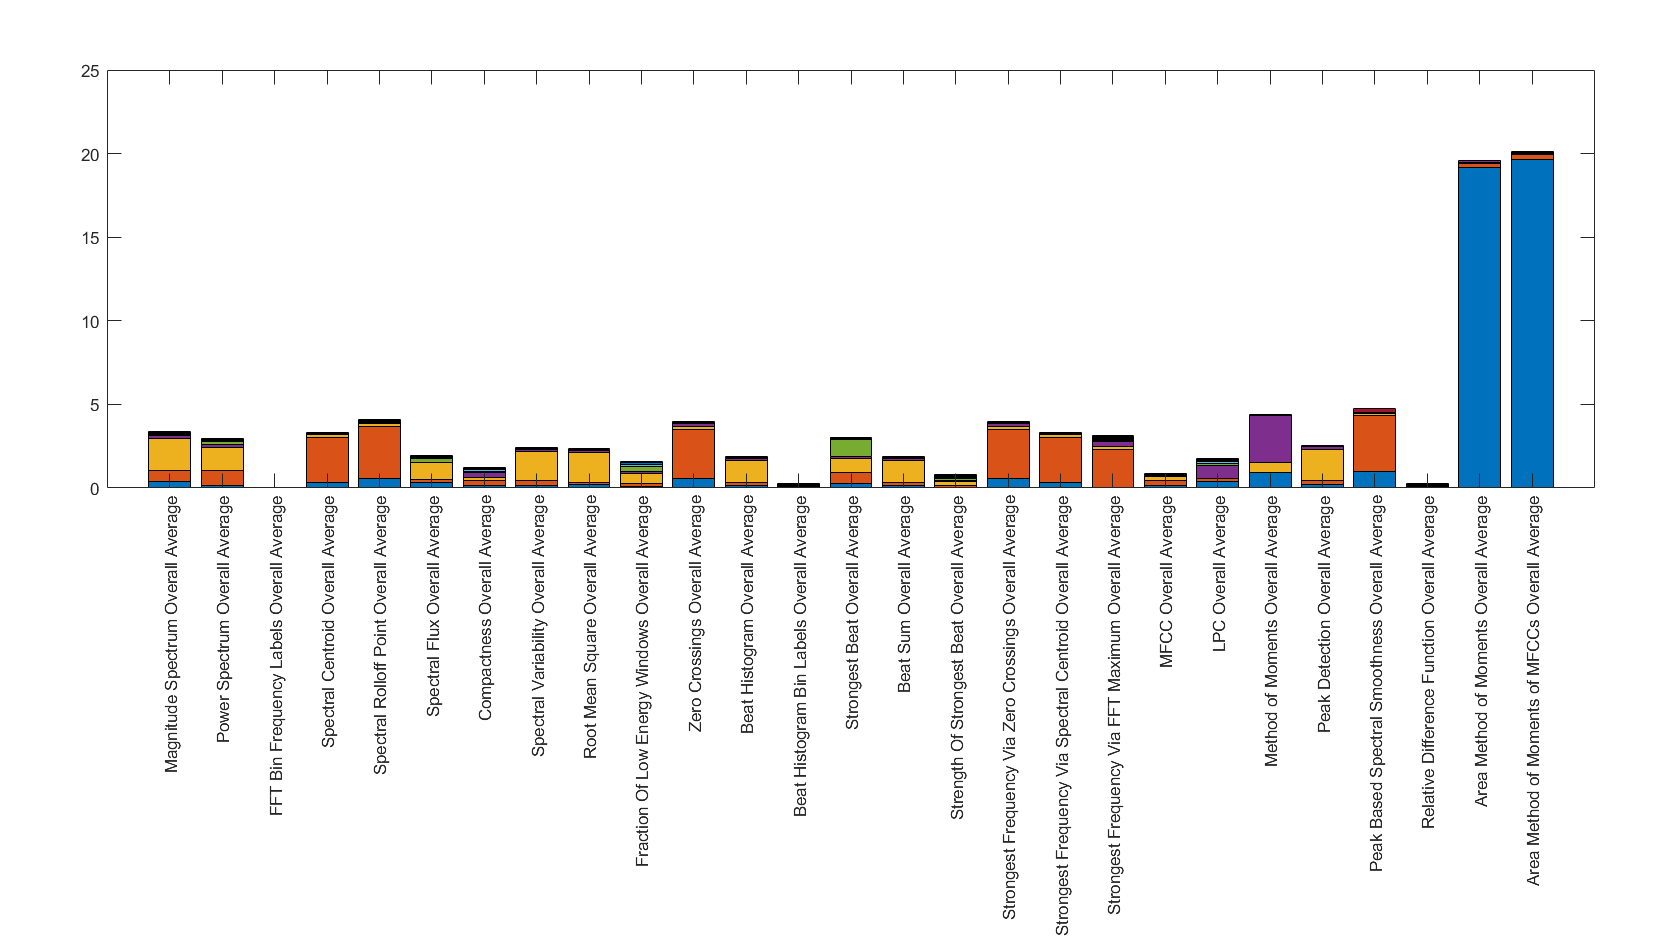
\includegraphics[scale=0.35]{pca_coeff_re.png}
    \caption{PCA coefficients weighted by eigen values (Normalized by Rescaling)}
    \label{fig:pca_coeff_re}
\end{figure}